\ifthenelse{\equal{\training}{linux-kernel}}{
  \begin{frame}
  \frametitle{Origin}
  \begin{columns}
    \column{0.8\textwidth}
    \begin{itemize}
    \item The Linux kernel was created as a hobby in 1991 by a Finnish
      student, Linus Torvalds.
      \begin{itemize}
      \item Linux quickly started to be used as the kernel for free
        software operating systems
      \end{itemize}
    \item Linus Torvalds has been able to create a large and dynamic
      developer and user community around Linux.
    \item As of today, about 2,000+ people contribute to each kernel
      release, individuals or companies big and small.
    \end{itemize}
    \column{0.2\textwidth}
      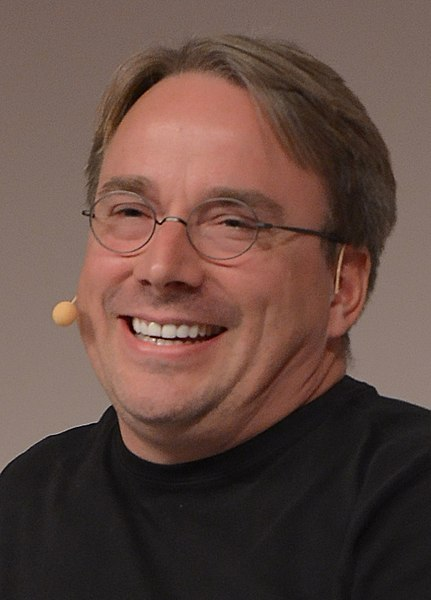
\includegraphics[width=\textwidth]{slides/sysdev-linux-intro-features/linus-torvalds.jpg}
      \scriptsize
      Linus Torvalds in 2014\\
      \tiny
      Image credits (Wikipedia):\\
      \url{https://bit.ly/2UIa1TD}
    \end{columns}
\end{frame}
}{}

\begin{frame}
  \frametitle{Linux kernel in the system}
  \begin{center}
    \includegraphics[height=0.8\textheight]{slides/sysdev-linux-intro-features/linux-kernel-in-system.pdf}
  \end{center}
\end{frame}

\begin{frame}{Linux kernel main roles}
  \begin{itemize}
  \item {\bf Manage all the hardware resources}: CPU, memory, I/O.
  \item Provide a {\bf set of portable, architecture and hardware
      independent APIs} to allow user space applications and libraries
    to use the hardware resources.
  \item {\bf Handle concurrent accesses and usage} of hardware
    resources from different applications.
    \begin{itemize}
    \item Example: a single network interface is used by multiple
      user space applications through various network connections. The
      kernel is responsible for ``multiplexing'' the hardware resource.
    \end{itemize}
  \end{itemize}
\end{frame}

\begin{frame}
  \frametitle{System calls}
  \begin{columns}
    \column{0.7\textwidth}
    \begin{itemize}
    \item The main interface between the kernel and user space is the set
      of system calls
    \item About 400 system calls that provide the main kernel services
      \begin{itemize}
      \item File and device operations, networking operations,
        inter-process communication, process management, memory mapping,
        timers, threads, synchronization primitives, etc.
      \end{itemize}
      \ifthenelse{\equal{\training}{linux-kernel}}{}{
      \item This interface is stable over time: only new system calls can
        be added by the kernel developers
      }
    \item This system call interface is wrapped by the C library, and
      user space applications usually never make a system call directly
      but rather use the corresponding C library function
    \end{itemize}
    \column{0.3\textwidth}
      \includegraphics[width=\textwidth]{slides/sysdev-linux-intro-features/system-calls.pdf}
      \scriptsize
      Image credits (Wikipedia):\\
      \url{https://bit.ly/2U2rdGB}
    \end{columns}
\end{frame}

\begin{frame}
  \frametitle{Pseudo filesystems}
  \begin{itemize}
  \item Linux makes system and kernel information available in user
    space through {\bf pseudo filesystems}, sometimes also called {\bf
      virtual filesystems}
  \item Pseudo filesystems allow applications to see directories and
    files that do not exist on any real storage: they are created and
    updated on the fly by the kernel
  \item The two most important pseudo filesystems are
    \begin{itemize}
    \item \code{proc}, usually mounted on \code{/proc}: \\
      Operating system related information (processes, memory
      management parameters...)
    \item \code{sysfs}, usually mounted on \code{/sys}: \\
       Representation of the system as a tree of
       devices connected by buses. Information
       gathered by the kernel frameworks managing these devices.
    \end{itemize}
  \end{itemize}
\end{frame}
